\newpage
\section{Results and interpretation} \label{section:result}

We use the same code for the interpretation of all lines and the meaning of the different colors are presented bellow on the figure \ref{fig:legend}.

\begin{figure}[H]
    \centering
    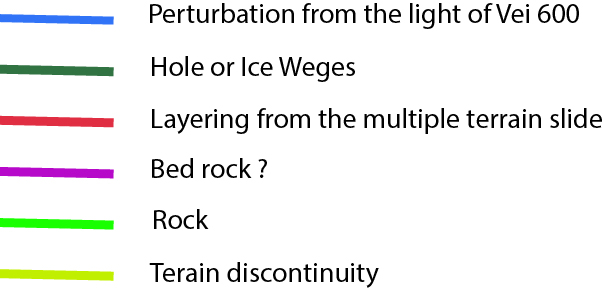
\includegraphics[width=0.5\linewidth]{Images/00_Results/Legend.jpg}
    \caption{Legend for the interpretation of the figure }
    \label{fig:legend}
\end{figure}


\subsection{Test survey}

For the test survey, survey to test the equipment, I went walking in the streets of Longyearbyen and found a very characteristics echo from pipes under the road.

\begin{figure}
    \centering
    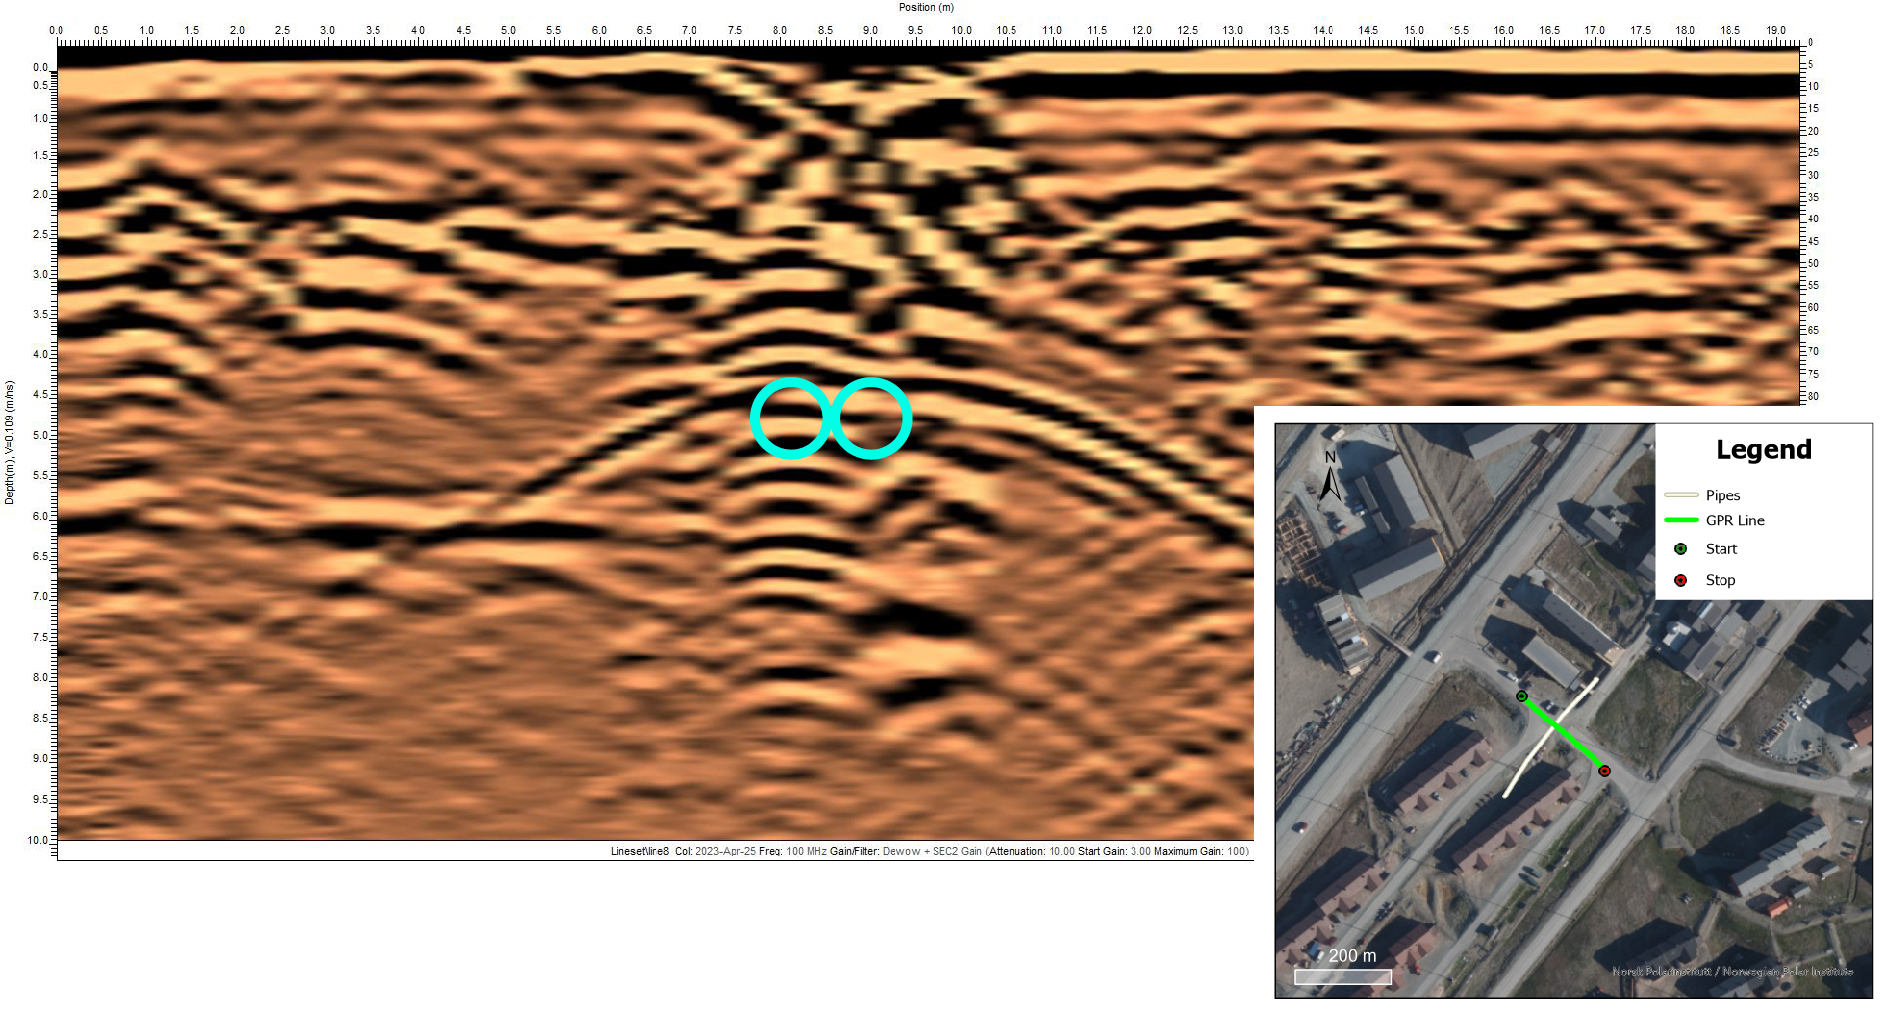
\includegraphics[width=\linewidth]{Images/00_Results/Test_line_edited.jpg}
    \caption{Test Line}
    \label{fig:testLine}
\end{figure}

The figure \ref{fig:testLine}, show a lot of small hyperbola around the position of the pipe which is very characteristics of single object buried. We also see some change in the upper layer due to the different material use for the road surface.


\subsection{Main Survey}

\begin{figure}
    \centering
    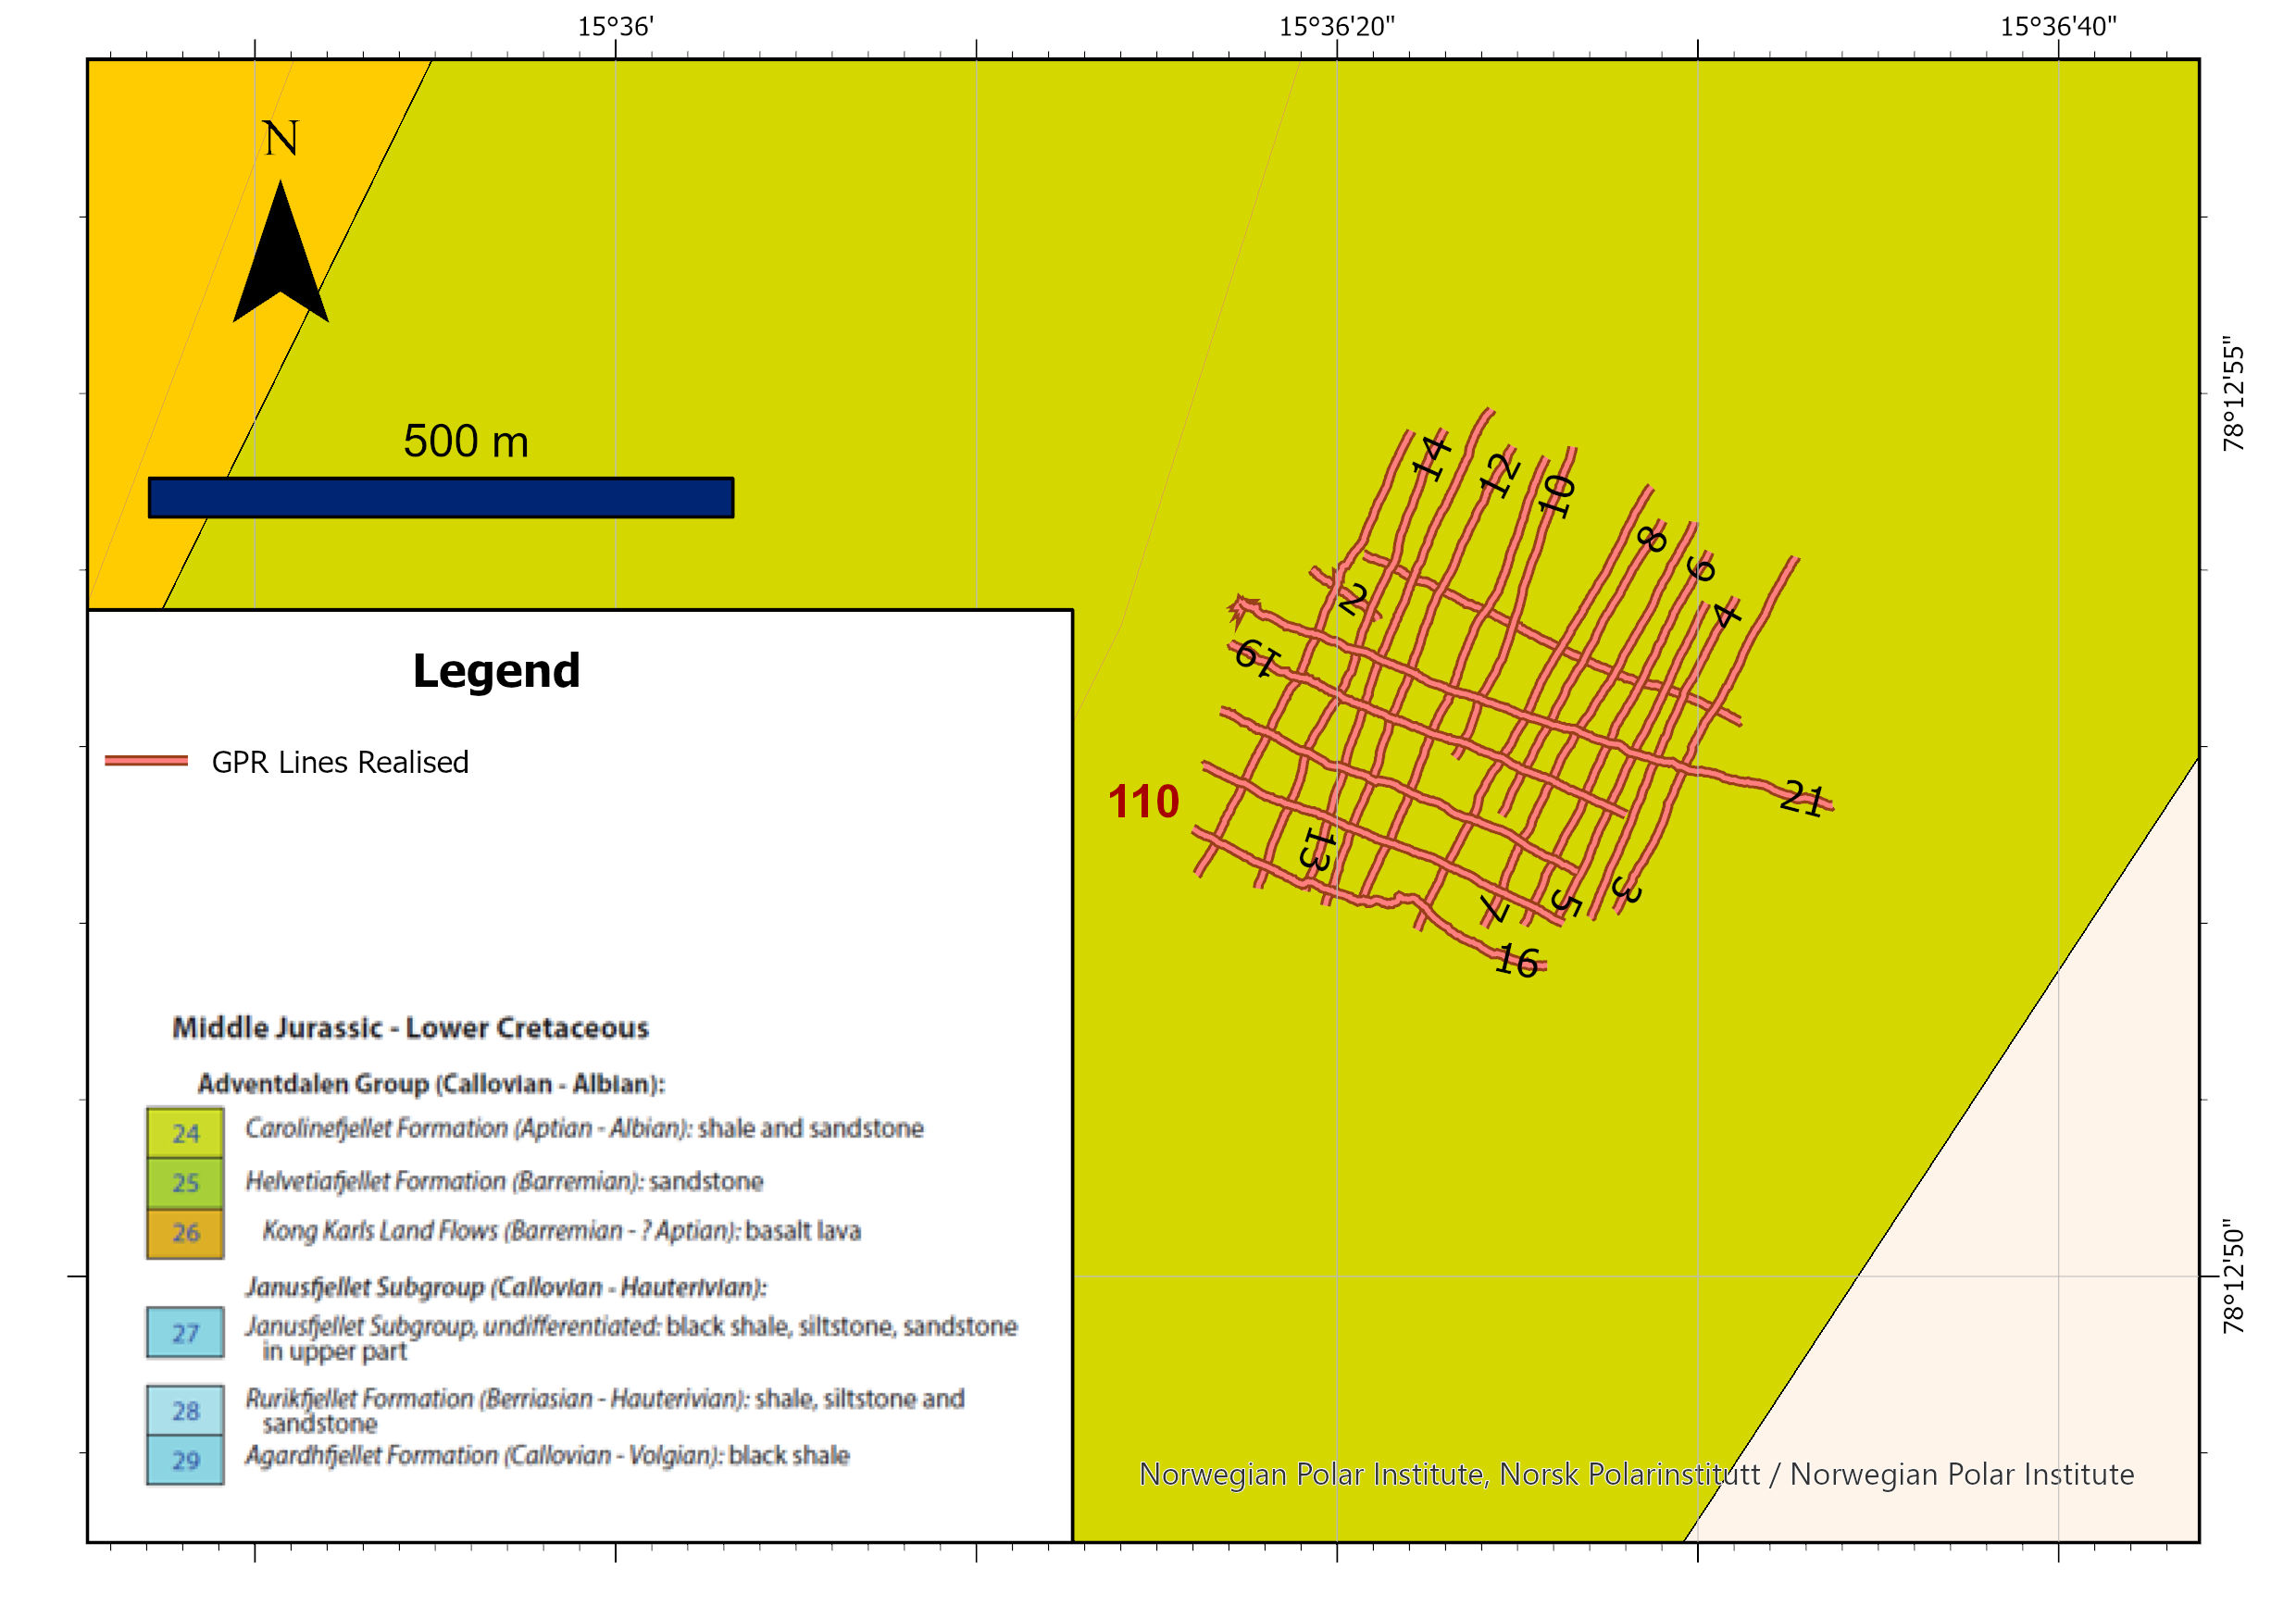
\includegraphics[width=\linewidth]{Images/00_Results/GPR LIne.jpg}
    \caption{Location of the different lines realised during the survey and number of the lines.}
    \label{fig:LocGPRLines}
\end{figure}

\paragraph{Results from the lines parallel to the slope} First we will present the lines realised parallel to the slope because they permit to understand some of the limitation of the GPR and of the ground. During that part, when start the line 2 and 20, the fiber optic of the receiver had some connection issue and so we restart the line and didn't processed it (because they was no data, just noise).

On all the lines we easily see the layering of the upper sedimentary part of the subsurface. This layering is most likely link to the different land slide and avalanche deposit in this run out area. This layering might also be generated by some kind of interference with the pulk even if this second hypothesis is very unlikely because of the irregularity of the layering.

On the line 1 presented on the figure \ref{fig:line1}, we might be able to see the bed rock (pink annotation). It's with the line 19 (figure \ref{fig:line19}) the two figure where we could see and underground layer which could correspond to the base rock. This hypothesis must be confirmed with some data providing the depth of the base rock at this position (borehole, geological archives...) and I didn't manage to found such a documentation. So according to this data the bed rock might be at a depth around 20m.

The only very visible hyperbola we see in the all survey are close to the road. My best guess is that structure appear because of the electric perturbation due to the public light close to the road or with the metal structure of the snow scooter which was used to carry all the equipment to the survey area. 

Unfortunately, it was the only good hyperbola to compute the velocity underground and so we get a velocity of $0.235m/ns$ which is quite high according to the velocity we could expect for permafrost area \cite{GPRAnalysis}.

Finally, we have some structure which are quite complicated to understand. My better guess is that structure could be some ice wedges as we capture in Adventdalen during the semester \cite{UNIS211-GPRReport}.

\begin{figure} [p]
    \centering
    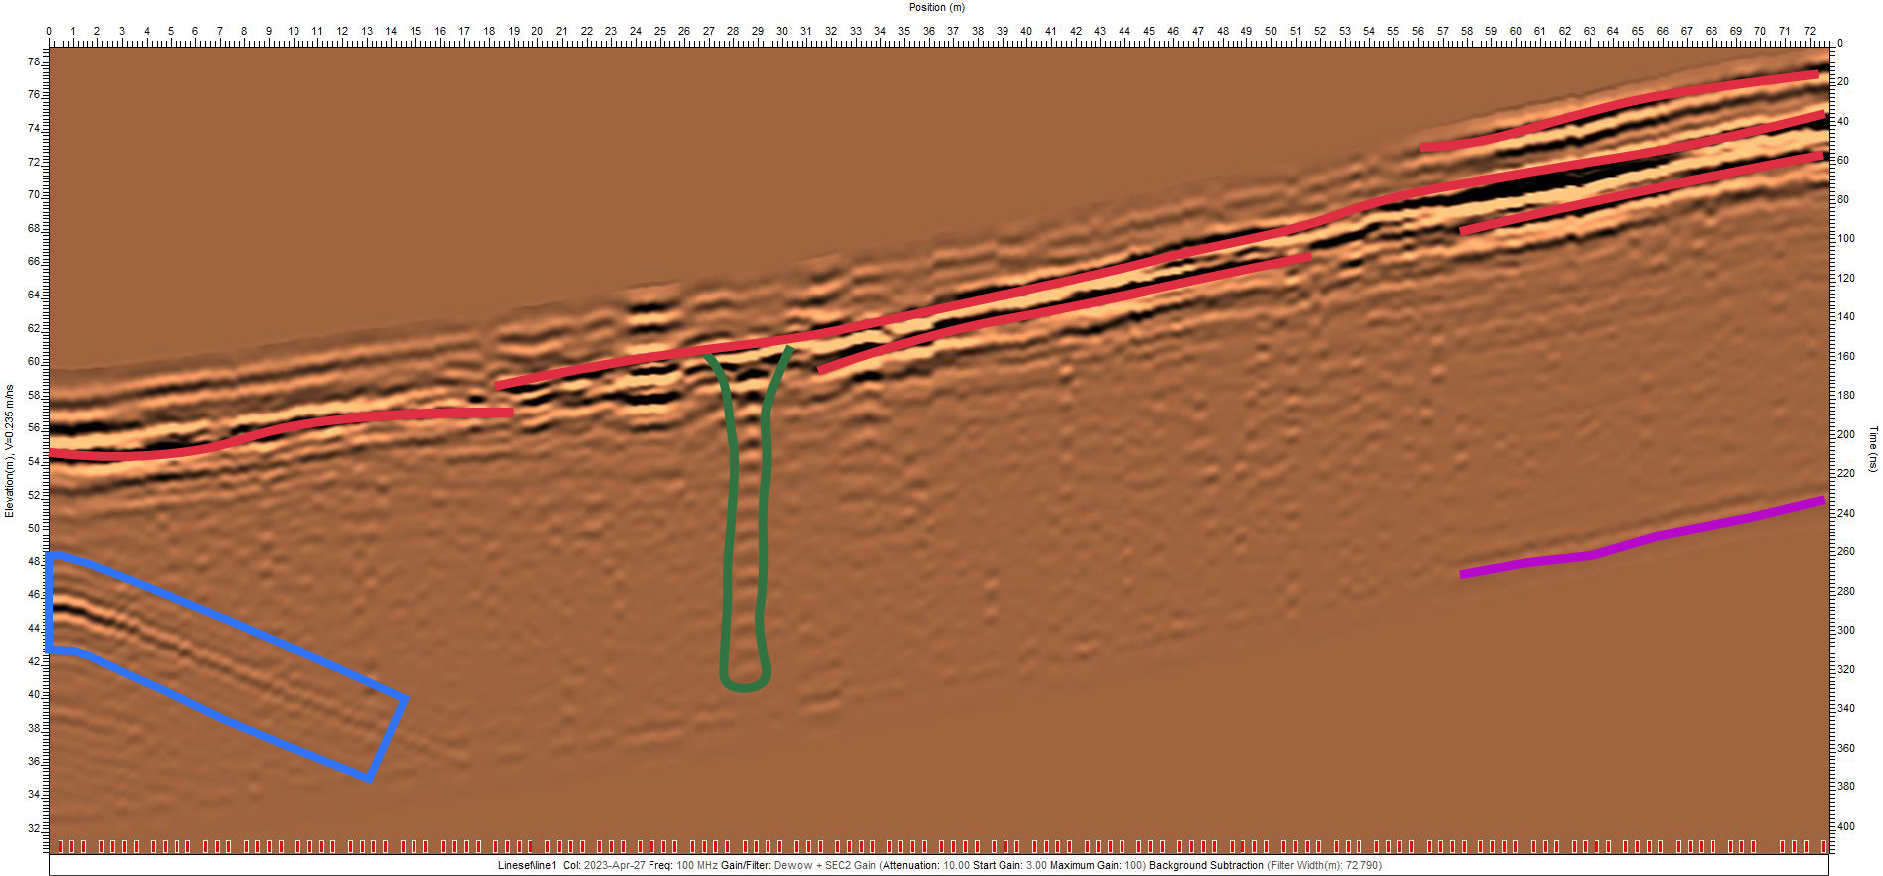
\includegraphics[width=\linewidth]{Images/00_Results/line1_edited.jpg}
    \caption{Line 1 with interpretations, legend on the figure \ref{fig:legend}}
    \label{fig:line1}
\end{figure}

\begin{figure}[p]
    \centering
    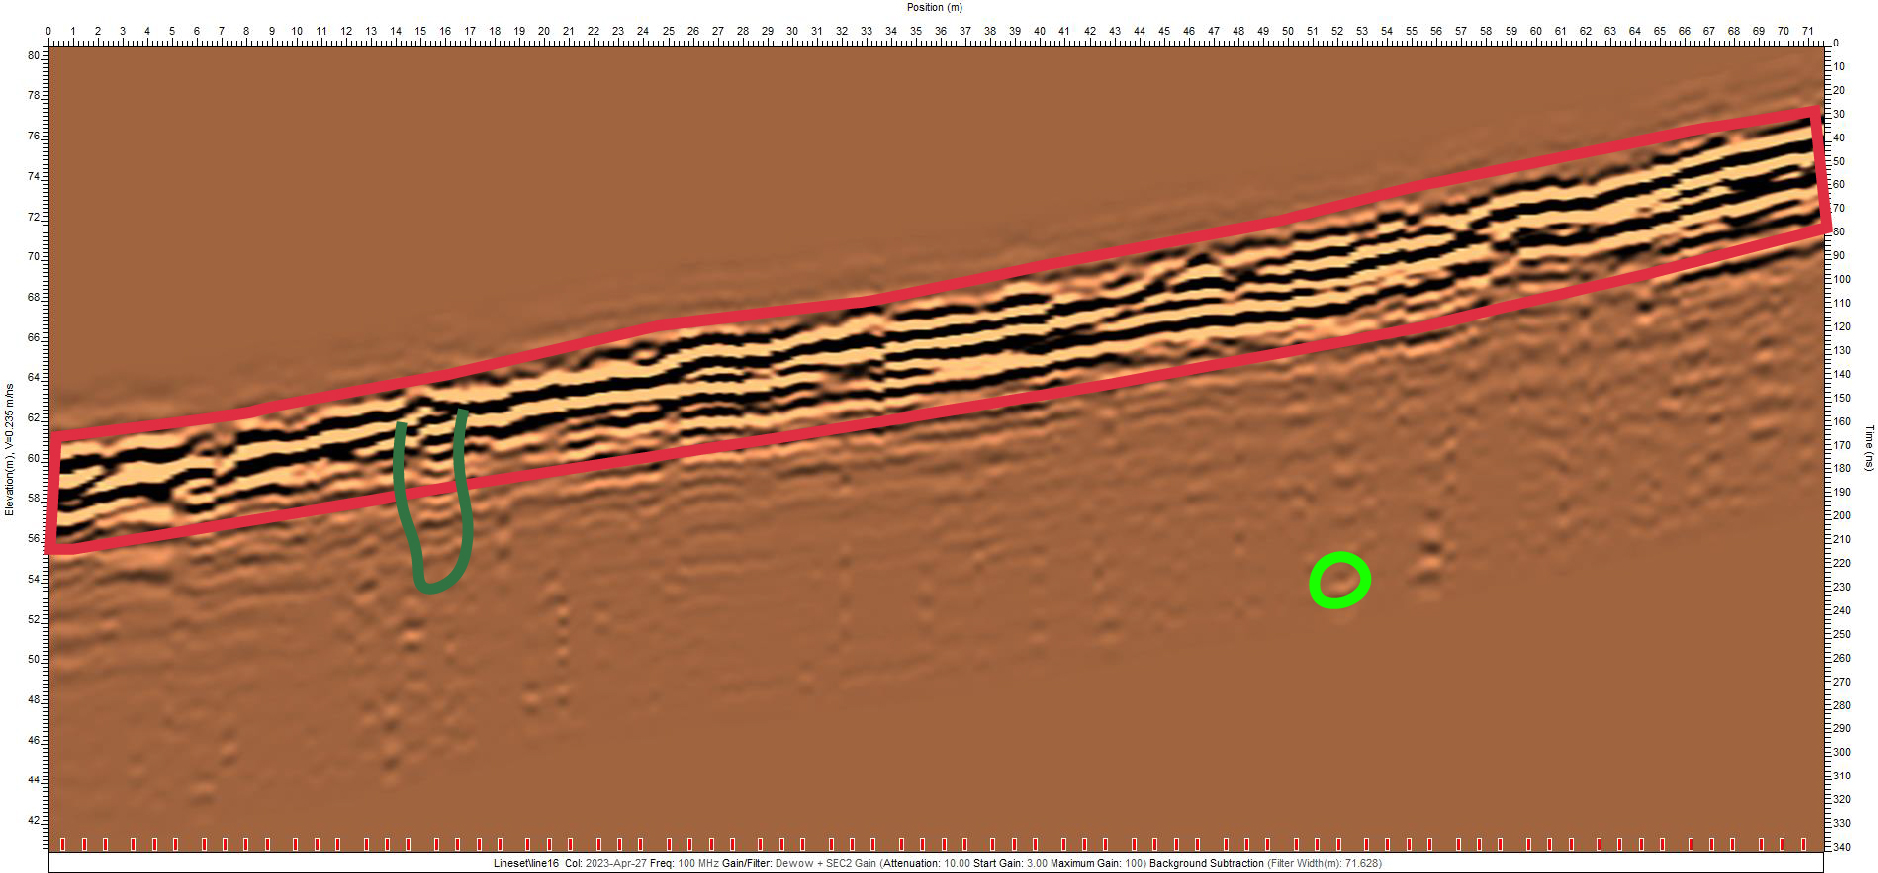
\includegraphics[width=\linewidth]{Images/00_Results/line16_edited.jpg}
    \caption{Line 16 with interpretations, legend on the figure \ref{fig:legend}}
    \label{fig:line16}
\end{figure}

\begin{figure}[p]
    \centering
    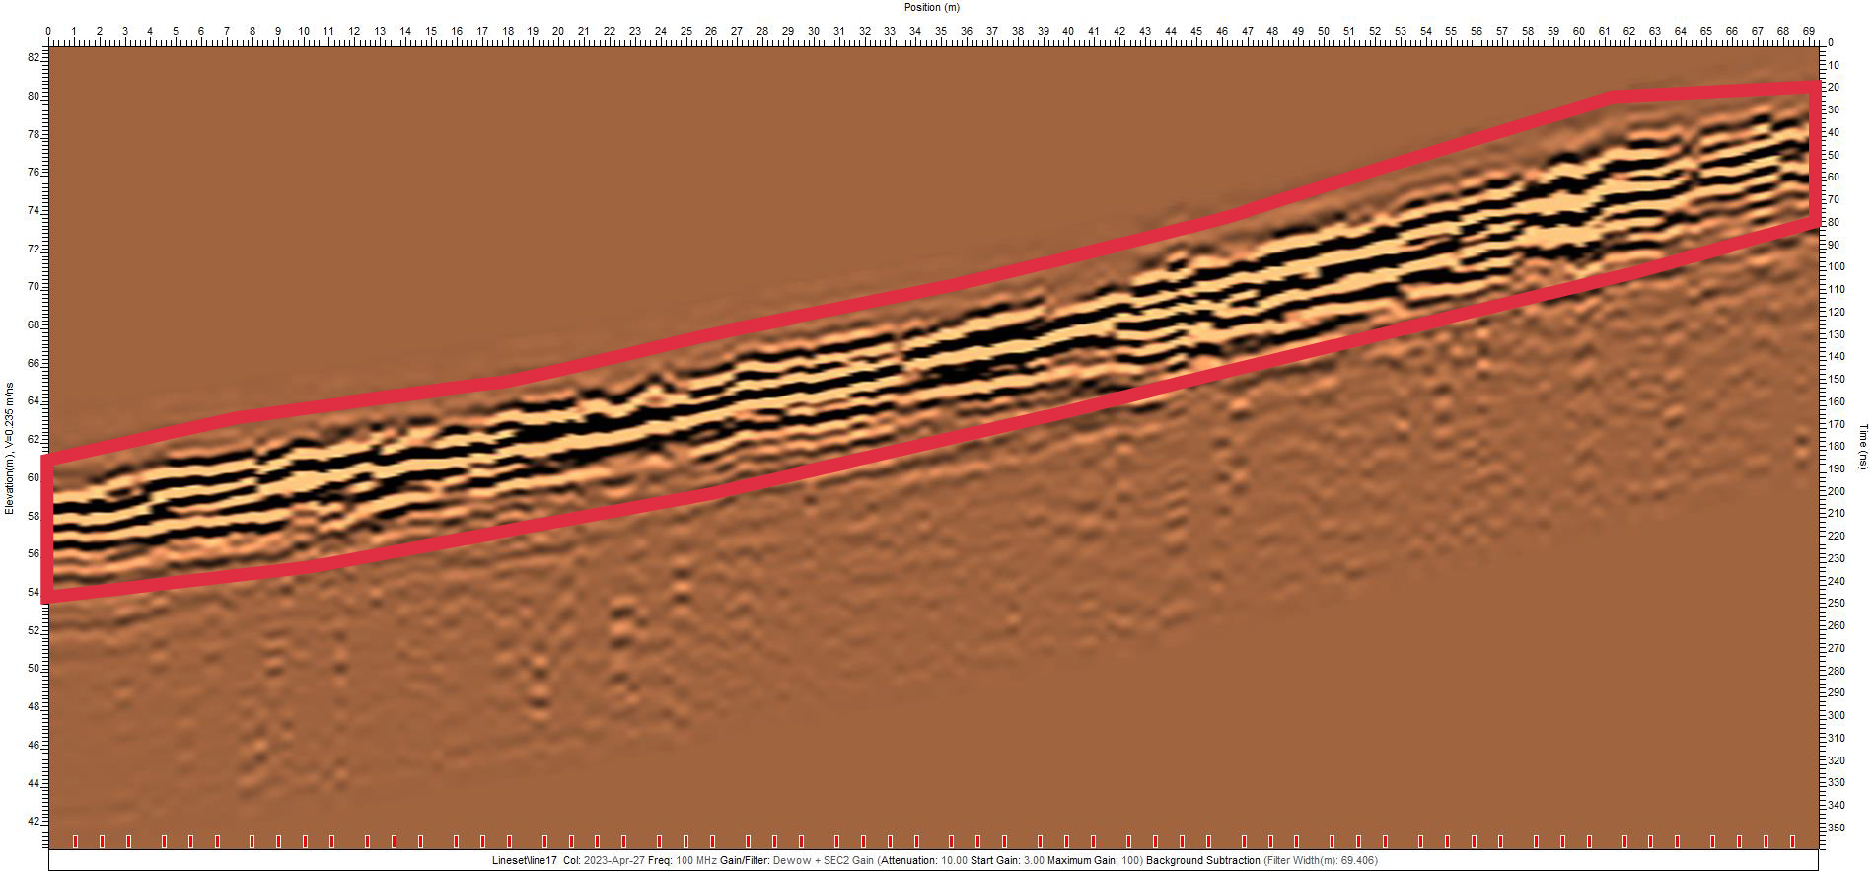
\includegraphics[width=\linewidth]{Images/00_Results/line17_edited.jpg}
    \caption{Line 17 with interpretations, legend on the figure \ref{fig:legend}}
    \label{fig:line17}
\end{figure}

\begin{figure}[p]
    \centering
    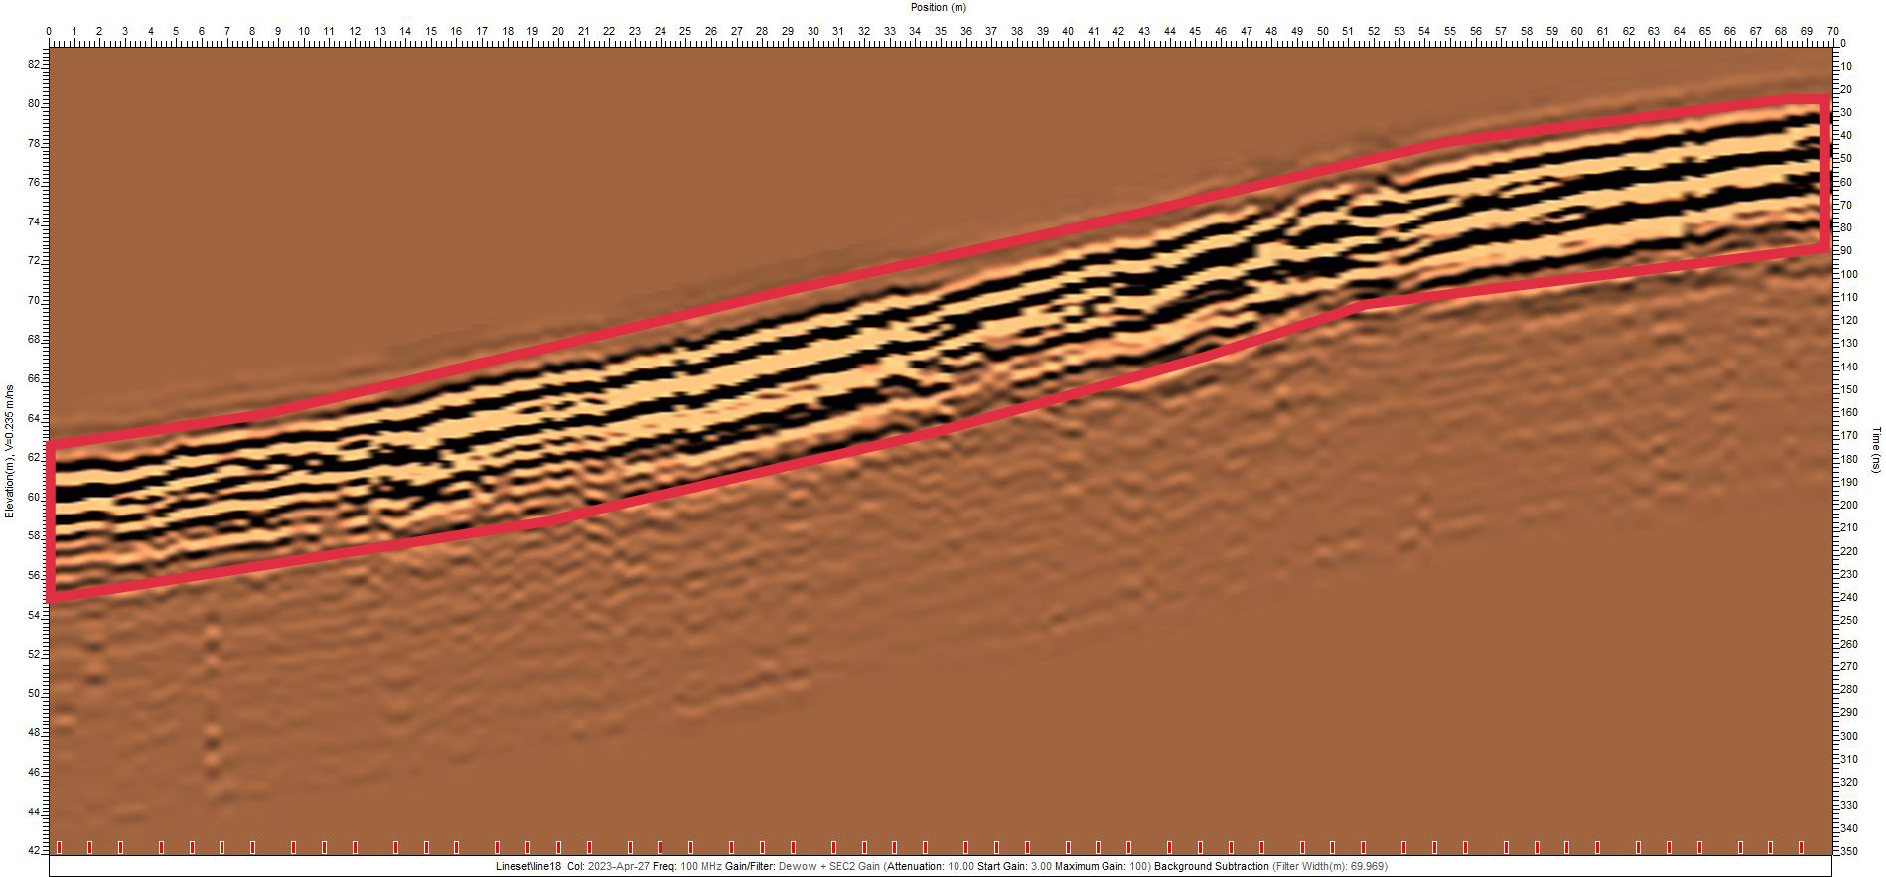
\includegraphics[width=\linewidth]{Images/00_Results/line18_edited.jpg}
    \caption{Line 18 with interpretations, legend on the figure \ref{fig:legend}}
    \label{fig:line18}
\end{figure}

\begin{figure}[p]
    \centering
    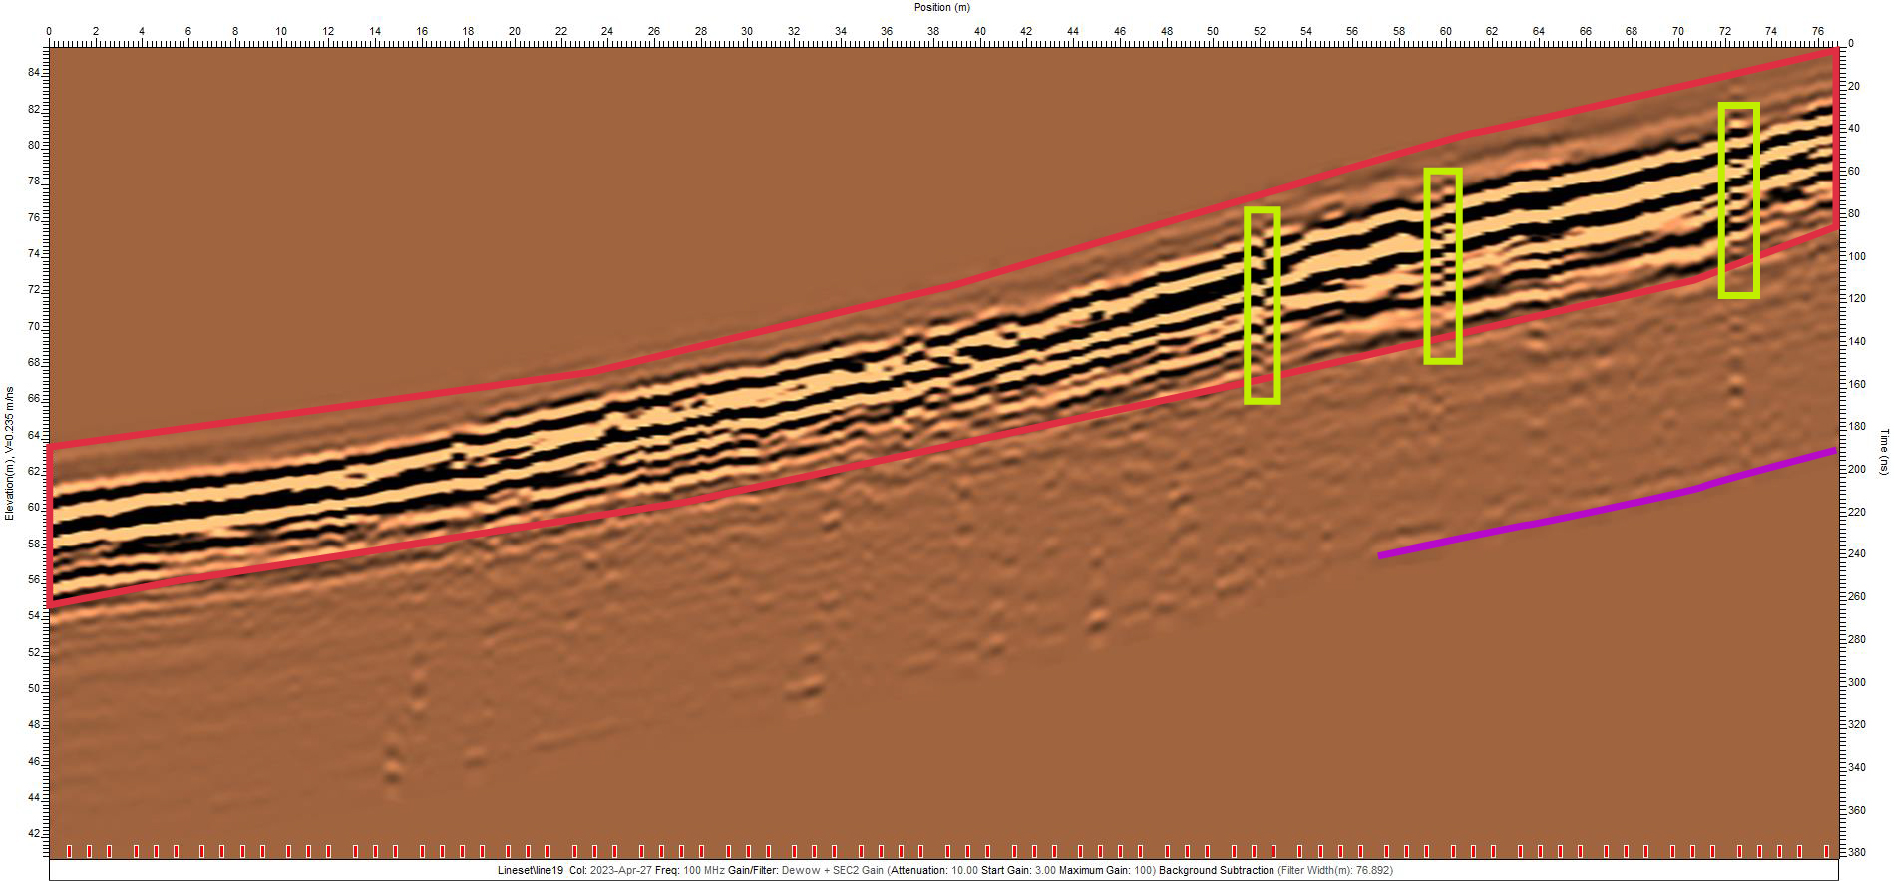
\includegraphics[width=\linewidth]{Images/00_Results/line19_edited.jpg}
    \caption{Line 19 with interpretations, legend on the figure \ref{fig:legend}}
    \label{fig:line19}
\end{figure}

\begin{figure}[p]
    \centering
    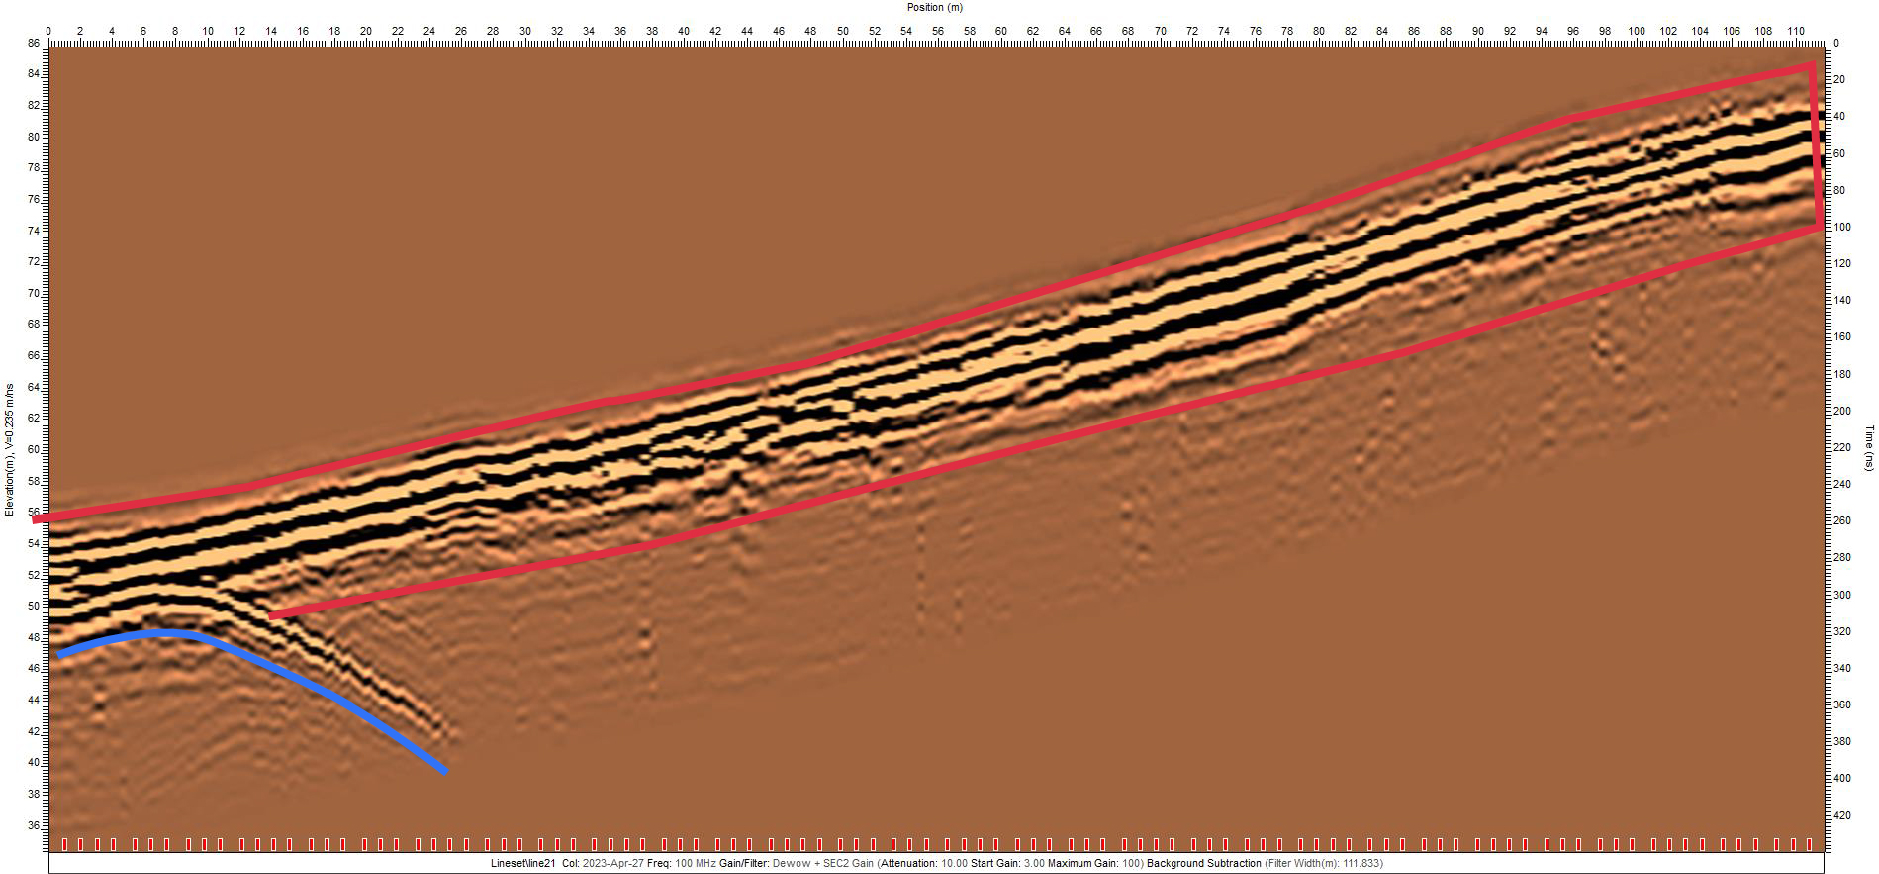
\includegraphics[width=\linewidth]{Images/00_Results/line21_edited.jpg}
    \caption{Line 21 with interpretations, legend on the figure \ref{fig:legend}}
    \label{fig:line21}
\end{figure}

